\documentclass{article}
\usepackage{amsmath}
\usepackage{graphics}
\usepackage{hyperref}
\usepackage[pdftex]{graphicx} % with the driver option
\title{Contact with CMB observations}
\author{Arthur Adriaens}
\date{\today}
\setcounter{section}{-1}

\begin{document}
	\maketitle

  \section{Introduction}
  We saw in the inflation notes that slow-roll inflation gives rise to gaussian fluctuations. We first discussed adiabatic density perturbations, these are scalar modes which are generated when they're super-horizon (super-Hubble) by a single time-shifting function. And as long as they're super-Hubble they satisfy
  \begin{equation}
    \delta = \delta_b = \frac{3}{4}\delta_\nu=\frac{3}{4}\delta_\gamma
  \end{equation}
  Where
  \begin{equation}
    \delta_x = \frac{\delta\rho_x}{\rho_x^{(0)}}
  \end{equation}
  (no index means dark matter)\\
  Now for super-Hubble scales during
\begin{itemize}
  \item radiation domination we saw that the gravitational potential was given by $\Psi = -\frac{1}{2}\delta_\gamma = const$
  \item matter domination: $\Psi = -\frac{1}{2}\delta = const$
\end{itemize}
These perturbations were characterized by a power spectrum $k^3P_\Psi(k) \sim k^{n-1}$, with n the tilt/spectral index/slope and $n-1 = -4\epsilon -2\delta$.\\
The second type of gaussian fluctuations correspond to gravitational waves (tensor modes), their spectrum is given by $k^3P_h(k)\sim k^{n_T}$ with $n_T = -2\epsilon$. These set the initial conditions for further cosmological evolution.
The best know CMB observable is probably the power spectrum shown in figure \ref{power spectrum}
\begin{figure}
  \centering
  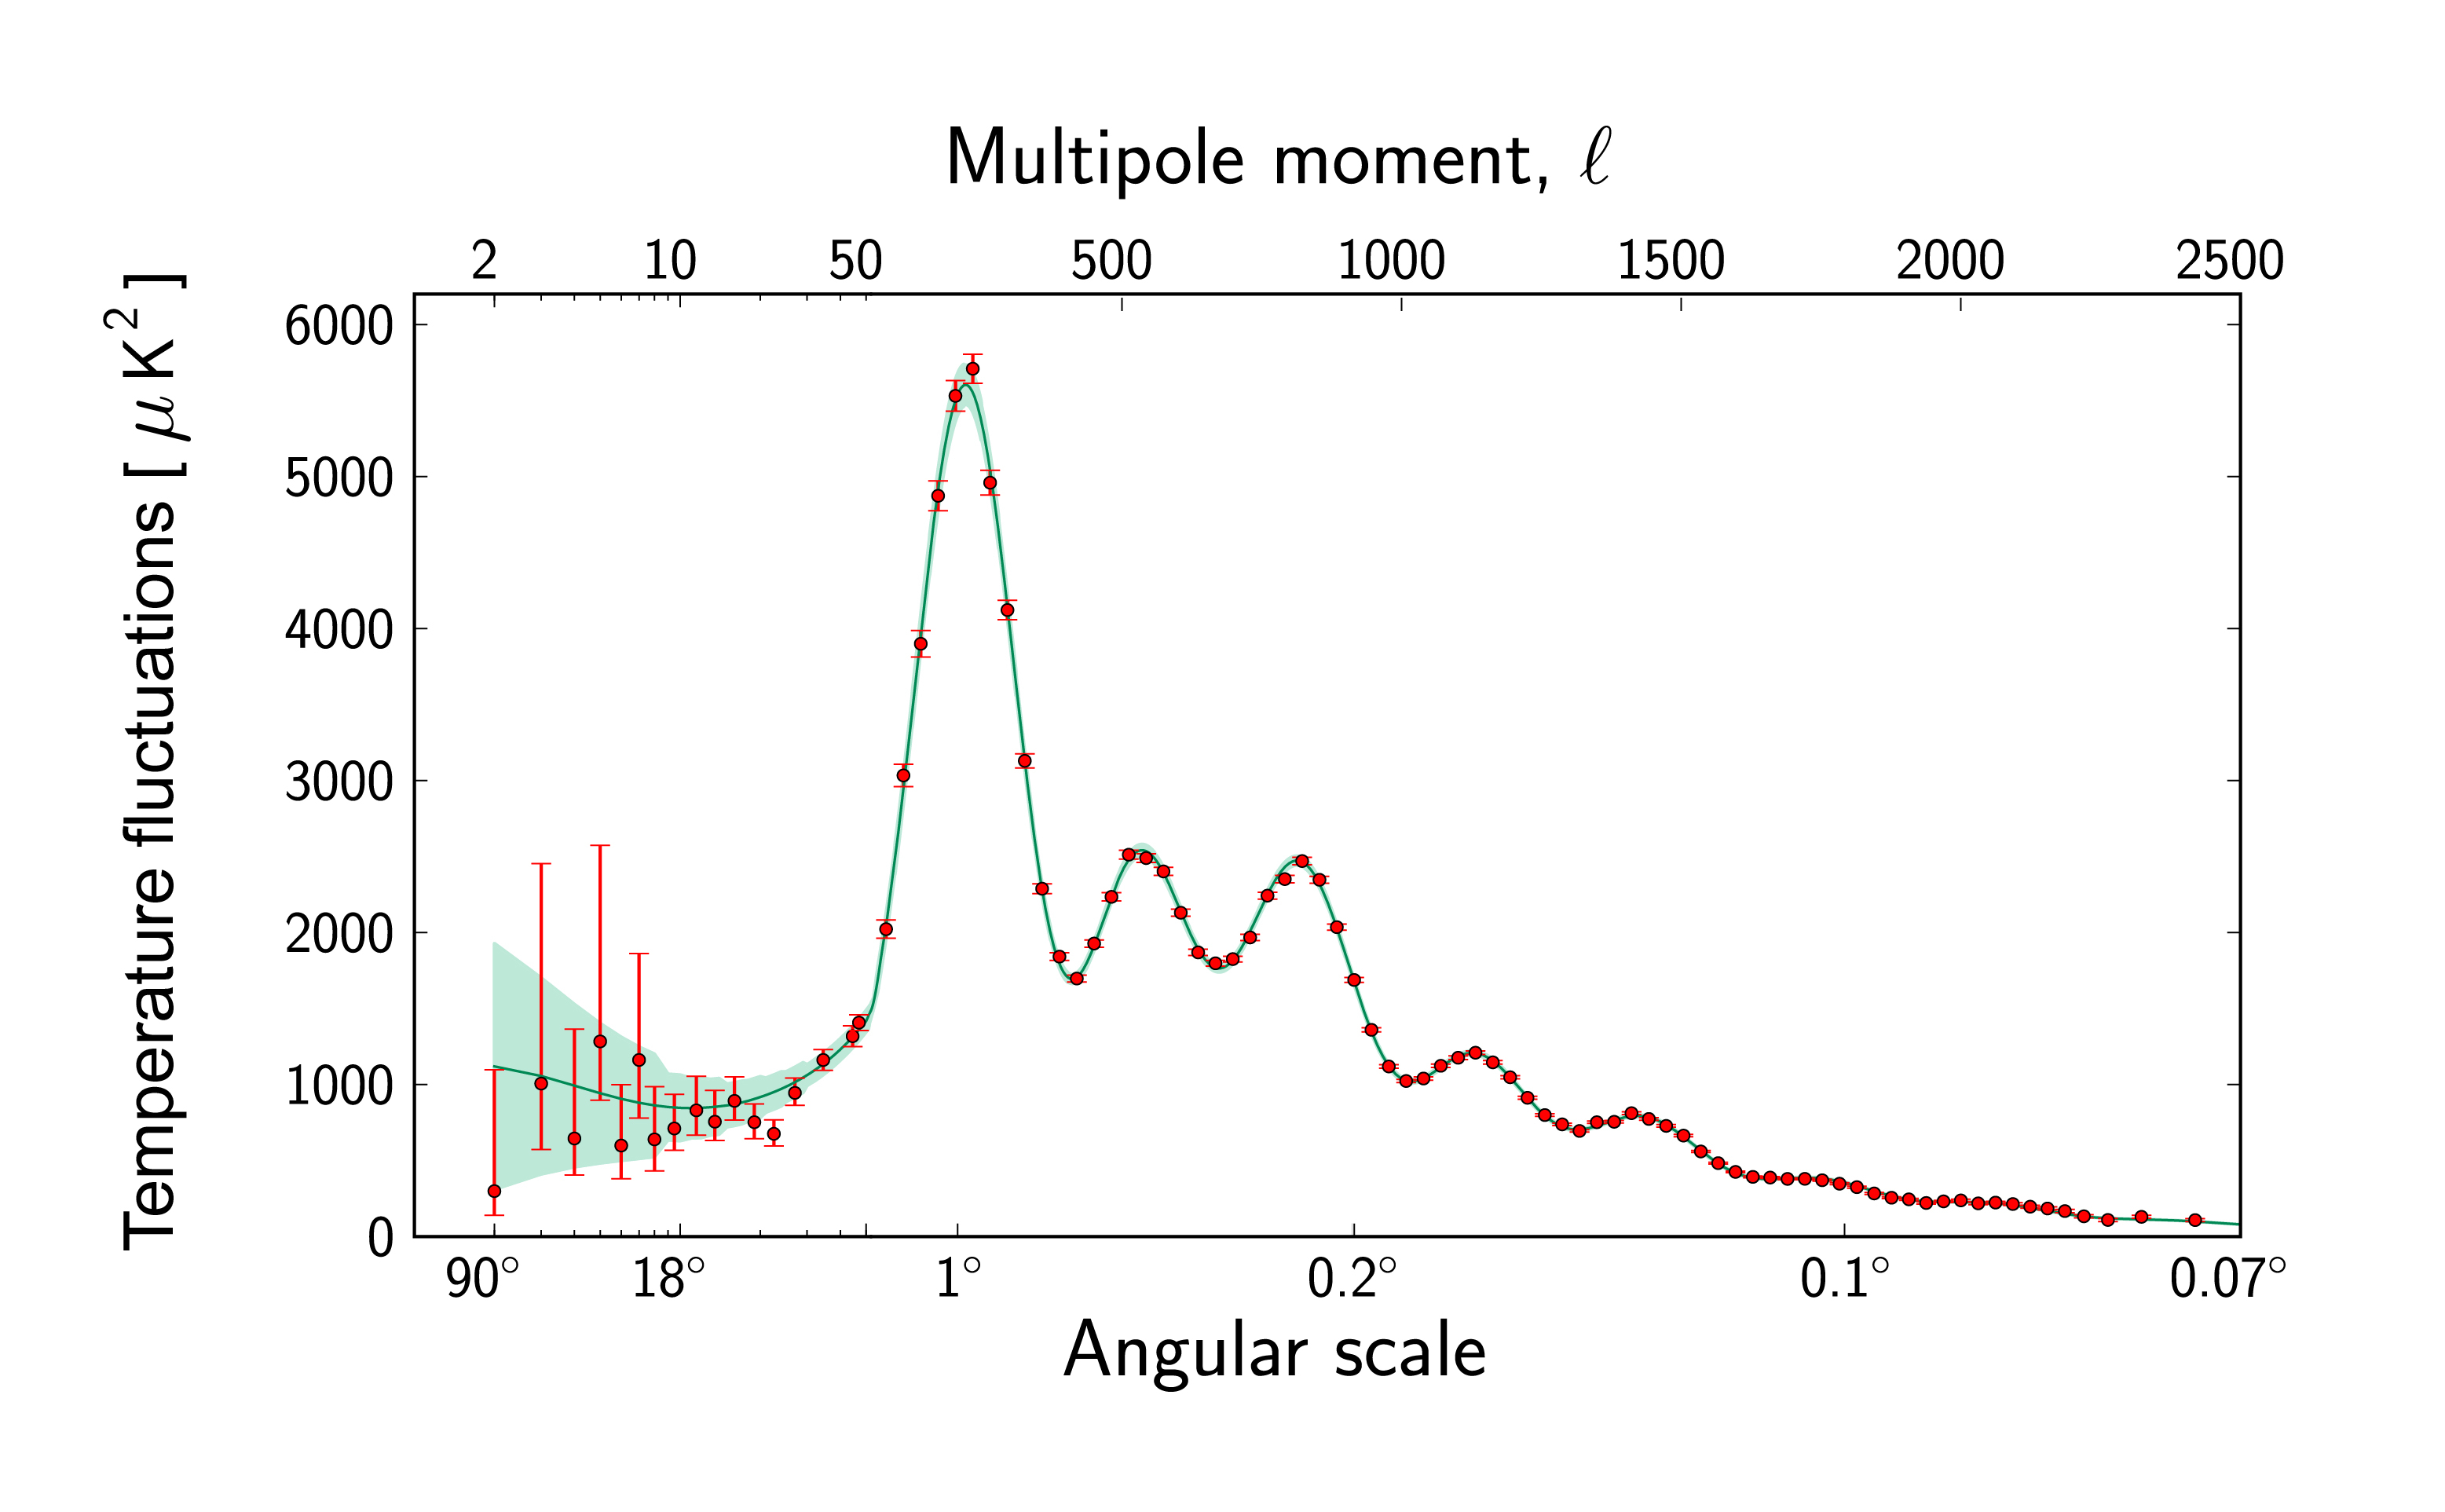
\includegraphics[width=0.8\textwidth]{Planck_power_spectrum_orig.jpg}
  \caption{CMB power spectrum}
  \label{power spectrum}
\end{figure}
 With the y-axis $l(l+1)C_l$ and the goal of this lecture is to understand the physics behind this. 
 \section{Photon scattering}
 An important ingredient to discuss in this story is photon scattering, we have photons which interact with electrons via thomson scattering, which in turn interact with baryons via Coulomb scattering. Coulomb scattering is alway very efficient $\implies$ electrons and baryons couple greatly to eachother. For Thomson scattering the story is a little different, to see wether Thomson scattering manages to keep photons and electrons in equilibrium we'll have to look at the thomson scattering rate (w.r.t conformal time):
\begin{equation}
   \Gamma = \sigma_T a n_e
\end{equation}
Now if we look at the behaviour of the thomson scattering rate as a function of redshift we see 2 important times: recombination/decoupling at z=1080 and reionization at $z\approx 10$:
\begin{figure}[h]
  \centering
  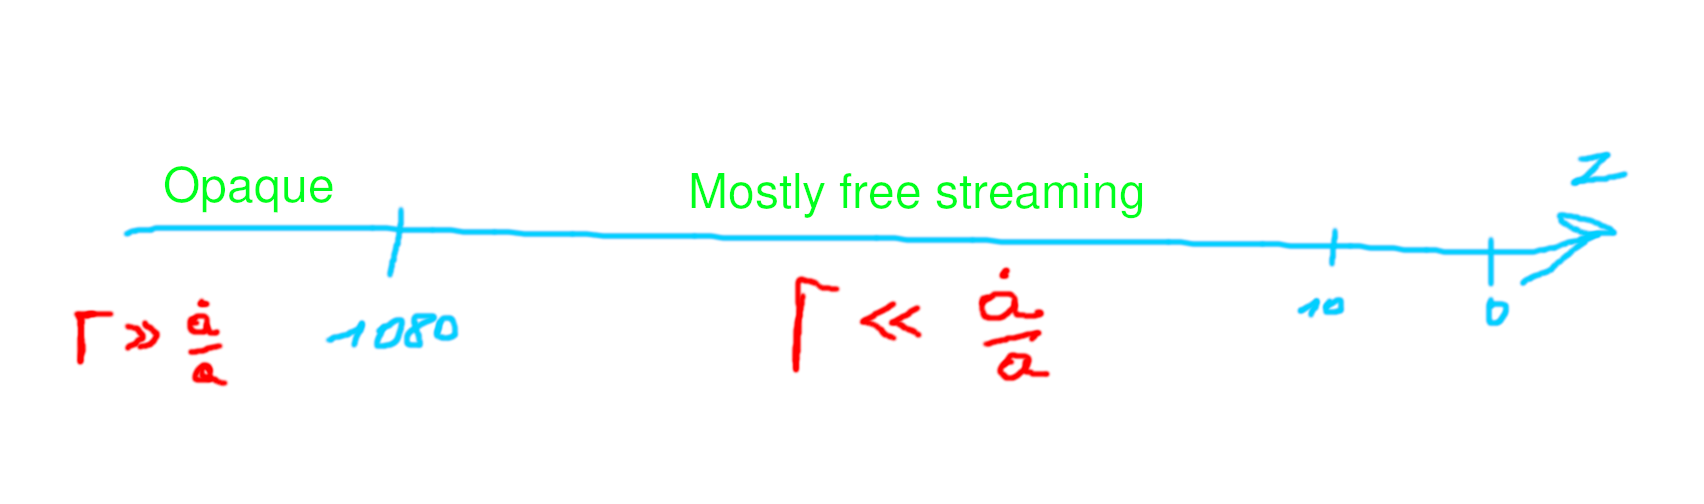
\includegraphics[scale=0.8]{universetimeline.png}
\end{figure}
Thomson scattering is way less efficient if they're bound to hydrogen and at reionization the universe was too diluted.\\\\
Another important concept here is the optical depth 
\begin{equation}
  \tau(\eta) \equiv \int_\eta^{\eta_0}d\tilde{\eta}\Gamma(\tilde{\eta})
\end{equation}
It can be interpreted as the opacity at a time $\eta$ when seen from today ($\eta = \eta_0$). And it corresponds to the expected number of scatterings of a photons since the time $\eta$. So one expects that $\tau\rightarrow \infty$ as $\eta\rightarrow 0$. $ \tau \approx 0.1$ between recombination and reionization and $\tau=0$ today.
\\\\
The next important concept is the visibility function:
\begin{equation}
  g(\eta) = -\dot{\tau}e^{-\tau}
\end{equation}
And corresponds to the probability density that a CMB photon seen today experienced last scattering at time $\eta$, we expect it to look like this:
\begin{figure}[h]
  \centering
  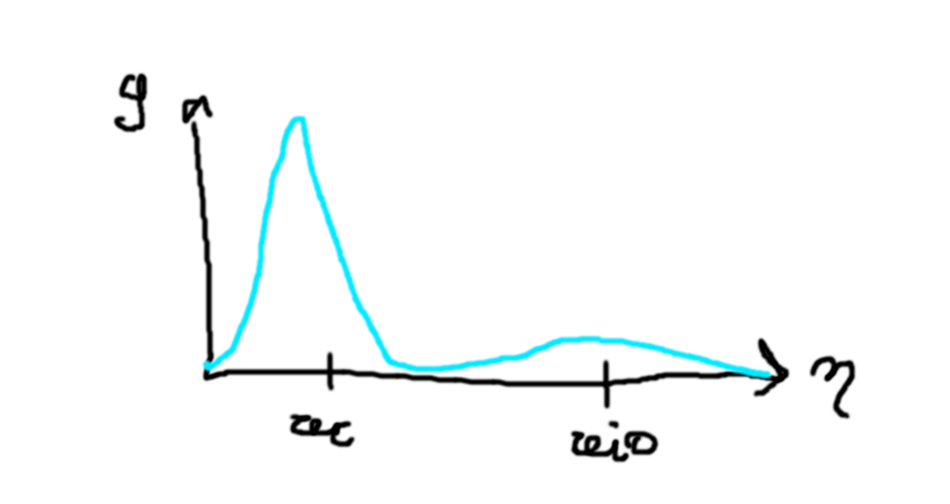
\includegraphics{visibility.png}
\end{figure}
The final important concept is the Diffusion length
\begin{equation}
  \lambda_d = a r_d
\end{equation}
Where $r_d$ is the comoving distance, now the comoving mean free path of photons is $r_{mfp} = \frac{1}{\Gamma(\eta)}$ in natural units. And if we use that in the formula for a random walk we get:
\begin{align}
  r_d(\eta) &\sim \left[\int_0^\eta d\tilde{\eta}\Gamma r_{mfp}^2\right]^{1/2}\\
            &=  \left[\int_0^\eta d\tilde{\eta}\frac{1}{\Gamma(\tilde{\eta})}\right]^{1/2}
\end{align}
This is an important concept to us as we'll see that the photon diffusion that happens just before recombination will damp the small scale anisotropies in the cosmic microwave background.



 \section{Boltzmann equation for photons}
	When photons are no longer in equilibrium we need the Boltzmann equation to describe their evolution, first let's expand the photon distribution function about it's equilibrium value (Bose-Einstein):
	\begin{equation}
		f(\eta,\vec{x},\vec{p}) = \left[exp\left\{\frac{p}{\tau(\eta)[1+\Theta(\eta,\vec{x},p)]}\right\}-1\right]^{-1}
	\end{equation}
	At early times the photons where in local thermal equilibrium with the electrons, that implies that the temperature fluctuation $\Theta$ doesn't depend on the momentum of the photon but only on the position x: $\Theta(\eta,\vec{x})$.
	After decoupling there's no longer local thermal equilibrium but one can show that the geodesic equation implies that the Bose-Einstein equation is perserved except that the temperature now depends on the propagation direction: $\Theta(\eta,\vec{x},\hat{p}).$\\
	Boltzmann eq:
	\begin{equation}
	\frac{df}{d\eta} = C[f,f_e]
\end{equation}
C being a collision term due to Thomson scattering, this equation can be written in the following form:
\begin{equation}
	\dot{\Theta} + \hat{p}\cdot\vec{\nabla}\Theta + \dot{\Phi} + \hat{p}\cdot\vec{\nabla}\Psi = -\Gamma(\Theta-\Theta_0 - \hat{p}\cdot\vec{V}_e)
\end{equation}
Here $\Phi$ and $\Psi$ are the scalar gravitational potentials, $\vec{V}_e$ is the bulk velocity of the electrons (which is the same as the bulk velocity of the baryons) and $\Theta_0$ is the average over angles of $\Theta$ ($\Theta_0 \equiv \frac{1}{4\pi}\int d\Omega' \Theta(\eta,\vec{x},\hat{p})$).\\
Now at early times the compton scattering rate $\Gamma$ is huge, and because of the product on the right hand side the part between brackets is driven to zero, i.e 
\begin{equation}
	\Theta = \Theta_0 + \hat{p}\cdot\vec{V}_b \label{*}
\end{equation}
This should be compared to a perfect fluid which is determined by the energy density and the velocity. Now we'll make the assumption that the velocity is irrotational, i.e the velocity is the gradient of a scalar velocity potential.\\
Now let's fourrier transform the perturbation $\Theta \rightarrow \tilde{\Theta}(\eta,\vec{k},\hat{p})$, now we make the claim that the FT transform doesn't depend on $\vec{k}$ and $\hat{p}$ seperately but on $\vec{k}$ and $\hat{k}\cdot\hat{p}$. i.e
\begin{equation}
	\tilde{\Theta}(\eta,\vec{k},\hat{k}\cdot\hat{p})
\end{equation}
Proof:
\begin{enumerate}
	\item Irrotational velocity $\implies$ $\vec{V}\parallel\vec{k}$. Looking back at equation \ref{*}, we see that the only dependence on $\hat{p}$ is on the combination $\hat{p}\cdot\vec{V}_b$ which is the same as $V_b \hat{p}\cdot\hat{k}$. So the claim holds at early times.
	\item The evolution equation only depends on $\hat{p}$ via the combination $\hat{p}\hat{k}$ which is a consequency of isotropy, therefore the claim continues to hold.
\end{enumerate}
Because of this we can expand $\tilde{\Theta}$ in Legendre polynomials:
\begin{equation}
	\tilde{\Theta}(\eta,\hat{k},\hat{k}\cdot\hat{p}) = \sum_l (-i)^l (2l + 1)\Theta_l(\eta,\vec{k})P_l(\hat{k}\cdot\hat{p})
\end{equation}
And at early times we know that we only have monopole and dipole contributions (l=0 and 1).
\section{Temperature anisotropy in a given direction}
To get some intuition for temperature anisotropies in the cosmic microwave background it's useful to start in a given direction. Let's consider the temperature anisotropy observed today when looking in a direction $\hat{p}$:
\begin{equation}
\frac{\delta T}{T}(\hat{p}) = \Theta(\eta_0,\vec{o},-\hat{p})
\end{equation}
The arguments are (now, here, photon moves in direction $-\hat{p}$). Now one can integrate the Boltzmann equation along the line of sight and one can use the approximation that recombination happens instantaneously (instantaneous decoupling) which means that the visibility function is given by a delta function: $g(\eta)=\delta(\eta-\eta_{dec})$. Which implies the following equation:
\begin{equation}
  (\Theta + \Psi)_{obs} = \left(\Theta_0 + \Psi + \hat{p}\cdot\vec{V}_b\right)\bigg|_{dec} + \int_{\eta_{dec}}^{\eta_0}d\eta (\dot{\Psi} - \dot{\Phi})
\end{equation}
The Theta on the left hand side can be interpreted as $\frac{\delta T}{T}(\hat{p})$ today, the subscript $_{obs}$ means at the observer location and along the line of sight, $\Theta_0$ is the temperature perturbation at recombination, $\hat{p}\cdot\vec{V}_b$ is a doppler correction due to the velocity of the baryon-photon fluid along the line of sight, $_{dec}$ refers to the last scattering surface along the line of sight. Then we have the gravitational potentials $\Psi$ on the left and right hand side (in obs and dec) and those can be interpreted as follows: if the potentials were constant in time there would be a gravitational redshift or blueshift which would depend on their difference
($\Psi\big|_{obs} - \Psi\big|_{dec}$). Finally we have an integral on the right hand side which is a non-conservative correction due to the time dependence of the potentials. The gravitational potential $\Psi$ on the left-hand side can be ignored in practice because it's a tiny isotropic correction (corresponds to a tiny shift in the temperature).
Given the last statement we can slightly re-write the equation in the following way:
\begin{equation}
  \Theta|_{obs} = \left(\Theta_0 + \Psi\right)\big|_{dec} + \hat{p}\cdot\vec{V}_b\big|_{dec} + \int_{\eta_{dec}}^{\eta_0}d\eta (\dot{\Psi} - \dot{\Phi})
\end{equation}
The first term on the right hand side is called the "Sachs-Wolfe (SW)" term, the second term is called the Doppler contribution and the last term is called the "integrated Sachs-Wolfe effect (ISW)".
It's instructive to first study this equation for large scales, e.g CMB maps smoothed over small scals (akin to bad resolution), then the temperature anisotropies are dominated by the SW term. The contributions to this SW term come from super-Hubble modes at the time of decoupling (Doppler negligable and ISW small).\\
Let's first consider $\Theta_0\big|_{dec}$, when the photons were in equilibrium thermodynamics says:
\begin{equation}
  \rho_\gamma \propto T^4 \implies \delta_\gamma = \frac{\delta\rho_\gamma}{\rho_\gamma} = \frac{4\delta T}{T} = 4\Theta_0
\end{equation}
Where $\delta T$ is averaged over all directions. Next consider $\Psi\big|_{dec}$, on super-Hubble scales for adiabatic initial conditions we know that:
\begin{equation}
  \delta_\gamma = \frac{4}{3}\delta_b
\end{equation}
And for super-Hubble scales during matter domination:
\begin{equation}
  -2\Psi = \delta_{tot} = \delta_b = \delta
\end{equation}
(both seen in the inflation notes) \\
If we bring all of this together then we find that on the last scattering surface:
\begin{equation}
  \Theta_0 + \Psi = \frac{1}{4}\delta_\gamma + \Psi = \frac{1}{4}(-2)\frac{4}{3}\Psi + \Psi = -\frac{2}{3}\Psi + \Psi = \frac{1}{3}\Psi
\end{equation}
If we neglect the doppler and ISW contributions, you find:
\begin{equation}
  \Theta\big|_{obs,\text{ large scales}} \approx \frac{1}{3}\Psi\big|_{dec} = -\frac{1}{8}\delta_\gamma\big|_{dec}
\end{equation}
Note that in the combination ($\Theta_0 + \Psi$), both terms have opposite signs and it's actually the gravitational potential $\Psi$ that dominates over $\Theta_0$. This means that if you have an overdensity on the last scattering surface ($\delta_\gamma>0$) then you actually have a cold spot (rather than a hot spot) in the observed map ($\Theta < 0$)
\section{Spectrum of temperature anisotropies}
Studying photons coming from a given direction is useful to get some intuition but our theories don't make predictions for what happens in any specific direction. In order to link theory to experiment, we need to study the spectrum of temperature anisotropies.\\
First let's expand the temperature anisotropy in spherical harmonics:
\begin{equation}
  \frac{\delta T}{T}(\hat{p}) = \Theta(\eta_0,\vec{0},-\hat{p}) = \sum_{lm}a_{lm}Y_{lm}(\hat{p})
\end{equation}
And using the addition theorem for spherical harmonics:
\begin{equation}
  P_l(-\hat{p}\cdot \hat{k}) = \frac{4\pi}{2l + 1}\sum_{m=-l}^l Y_{lm}(\hat{p})Y^*_{lm}(-\hat{k})
\end{equation}
We can write the temperature anisotropy as follows:
\begin{align}
  \Theta(\eta_0,\vec{o},-\vec{p}) &= \int \frac{d^3 k}{(2\pi)^3}\tilde{\Theta}(\eta_0,\vec{k},-\hat{p})\\
                                  &= \int \frac{d^3 k}{(2\pi)^3} \sum_l (-i)^l (2l + 1)\Theta_l(\eta_0,\vec{k})P_l(-\hat{p}\cdot\hat{k})\\
                                  &= \int \frac{d^3 k}{2\pi^2} \sum_{lm} (-i)^l\Theta_l(\eta_0,\vec{k}) Y_{lm}^*(-\hat{k})Y_{lm}(\hat{p})
\end{align}
i.e first: FT, second: Expand in Legendre polynomials and lastly we used the addition theorem. With this we find that $a_{lm}$ is given by:
\begin{equation}
  a_{lm} = (-i)^l \int \frac{d^3}{2\pi^2}Y_{lm}^*(-\hat{k})\Theta_l(\eta_0,\vec{k})
\end{equation}
Let's write $\Theta_l$ on the RHS in a convenient way:
\begin{equation}
  \Theta_l(\Theta_0,\vec{k}) = \zeta(\vec{k})\times \frac{\Theta_l(\eta_0,\vec{k})}{\zeta(\vec{k})}
\end{equation}
With $\zeta$ defined as in the inflation notes, interestingly the ratio on the RHS is independent of the initial conditions (as the evolution equation is linear) and it only depends on the magnitude of $\vec{k}$ and not it's orientation. This ratio is called the Transfer function. And $\zeta(\vec{k})$ is what we call the initial condition for the subsequent evolution of the universe after inflation. This initial condition is chosen during inflation from some gaussian distribution as in the inflation notes.\\
We define the transfer function as $\Theta_l(\eta_0,k)$ (we dropped the vector arrow). I.e we have seperated $\Theta_l(\eta_0,\vec{k})$ into something probabilistic ($\zeta$) which is determined during inflation, chosen from some probability distribution and a transfer function which can be computed using the evolution equation.\\
Now we're ready to compute the 2-point correlation function between the coëfficients:
\begin{align}
  <a_{lm}a^*_{l'm'}> &= (-i)^{l-l'}\int \frac{d^3 k}{2\pi^2}Y_{lm}^*(-\hat{k})\Theta_l(\eta_0,k)\\
                     &\qquad\qquad \times   \int \frac{d^3 k'}{2\pi^2}Y_{l'm'}(-\hat{k'})\Theta^*_{l'}(\eta_0,k')\\
                     &\qquad \qquad \times <\zeta(\vec{k})\zeta^*(\vec{k'})>
\end{align}
Now from the isotropic gaussian distributions we discussed in the notes on inflation we have that:
\begin{equation}
  <\zeta(\vec{k})\zeta^*(\vec{k'})> = (2\pi)^3 P_\zeta(k)\delta(\vec{k}-\vec{k'})
\end{equation}
filling this in we find that
\begin{equation}
  <a_{lm}a^*_{l'm'}> = \delta_{l,l'} \delta_{m,m'}C_l
\end{equation}
With
\begin{equation}
  C_l = \frac{2}{\pi}\int dk k^2 \left|\Theta_l(\eta_0,k)\right|^2 P_{\eta}(k)
\end{equation}
Where the kronicker delta's can be traced back to homogeneity and that $C_l$ doesn't depend on m can be traced back to isotropy. Now it's very important that the $C_l$'s do not depend on m, the $C_l$'s are the variances of a theoretical probability distribution for the $a_{lm}$'s but we only have acces to one temperature map, i.e one realisation of the probability distribution. So you might be worried that we don't have enough observational input to test the theoretical prediction, however because the $C_l$'s don't depend on m, we have the same variance for all the different m modes. So we do have some statistics to test the prediction and especially when l is large there are many values of m that we can use in order to test the predictions of our models. In fact the best estimate that we can come up with for $C_l$ is:
\begin{equation}
  C_l^{obs} \equiv \frac{1}{2l + 1} \sum_{m=-l}^l |a_{lm}^{obs}|^2
\end{equation}
I.e the average of all the observed modulus squared values. And in this way we can see that cosmic variance will be very important for small values of l which correspond to large features on the sky.\\\\
When we were talking about anisotropies in a certain direction a starting point was a line-of-sight integral in position space, we can now do one in momentum space with as a result:
\begin{align}
  \Theta_l(\eta_0,k) &\approx \left[\Theta_0(\eta_{dec},k) + \Psi(\eta_{dec},k)\right]j_l\left[k(\eta-\eta_{dec})\right] \\
  &\quad + iV_b j'_l\left[k(\eta_0-\eta_{dec})\right]\\
  &\quad + \int_{\eta_{dec}}^{\eta_0} d\eta\left[\dot{\Psi}(\eta,k) - \dot{\Phi}(\eta,k)\right]j_l\left[k(\eta_0-\eta)\right]
\end{align}
We find 3 terms as before, again called (in order) SW, Doppler and ISW contribution. As this quantity appears squared in $C_l$, $C_l$ consists of 6 terms: $C_l^{SW}$, $C_l^{Doppler}$, $C_l^{ISW}$ and the cross terms. Now for large l, the spherical bessel functions $j_l(x)$ and $j_l'(x)$ are peaked near $x\approx l$ which implies that the SW and Doppler contributions are dominated by
\begin{equation}
  k \approx \frac{l}{\eta_0 - \eta_{dec}}
\end{equation}
Which is an imortant relation as it implies that spatial scales at the decoupling respond to angular scales today.
We can, for instance, take this into account for the SW contribution to $C_l$:
\begin{equation}
  C_l^{SW} \sim \left|\Theta_0(\eta_{dec},k) + \Psi(\eta_{dec},k)\right|^2 P_\zeta (k)\big|_{k \approx \frac{l}{\eta_0 - \eta_{dec}}}
\end{equation}
\newpage
\section{Acoustic oscillations}
Before decoupling the photons and the baryons form a single fluid with sound speed
\begin{equation}
  c_s^2 = \frac{\delta p_\gamma + \delta p_b}{\delta \rho_\gamma + \delta \rho_b}
\end{equation}
Since the energy density in baryons goes like: $\rho_b \sim T^3$ and in photons $\rho_\gamma \sim T^4$ we have that $\delta_\gamma = \frac{4}{3}\delta_b$, we also know that pressure perturbations in baryons are much smaller than in photons: $|\delta p_b| \ll |\delta p_\gamma|$. Combining these equations we get for the speed of sound:
\begin{equation}
  c_s^2 = \frac{1}{3(1+R)}
\end{equation}
With
\begin{equation}
  R \equiv \frac{3\rho_b^{(0)}}{4\rho_\gamma^{(0)}} \quad (\sim a)
\end{equation}
Now we'll write down the equation of motion for the photon temperature fluctuations $\Theta_0(\eta,\vec{x})$ (l=0)  in this tightly coupled regime:
\begin{equation}
  \ddot{\Theta}_0 + \frac{\dot{R}}{1+R}\dot{\Theta}_0 + k^2c_s^2 \Theta_0 = -\frac{k^2}{3}\Psi - \frac{\dot{R}}{1+R}\dot{\Phi} - \ddot{\Phi} \label{oscillations}
\end{equation}
Since $R\sim a \implies \dot{R} = \frac{a}{a}R = aHR$. The second term (LHS) is a damping term and is stronger if there are more baryons, this is different from the diffusion damping (unrelated) and we'll ignore this term. The third term on the LHS represents pressure forces which give rise to accoustic oscillations. The first term on the RHS comes from the gravitational force and the last 2 terms correspond to dilation effects. Now an important concept related to this equation is that of the sound horizon:
\begin{equation}
  r_s(\eta) \equiv \int_0^\eta c_s(\tilde{\eta})d\tilde{\eta}
\end{equation}
And if we were to ignore damping and approximate $R$ as slowly varying then we would find as solution for the temperature perturbation:
\begin{equation}
  \Theta_0(\eta) = \Theta_0(0)\cos(kr_s(\eta)) + \text{gravitational corrections}
\end{equation}
This solution represents the "acoustic oscillations", it's important to note that the phase in the solution is fixed for all the modes by adiabatic initial conditions. Which says that $\Theta_0=\text{constant for }k\eta \ll 1 \implies$ all modes are in phase! So these modes oscillate as a function of time but the CMB is like a snapshot taken at the time of decoupling, so what are the most important modes for the CMB? Those would be the modes who're extremal at the time of decoupling $\eta_{dec}$: Peaks at $kr_s(\eta_{dec}) = n\pi \implies$ peaks on corresponding angular scales in CMB power spectrum. The relation between spatial and angular scales depends on the spatial curvature of the universe! (look at the angle in the image below)
\begin{figure}[h]
  \centering
  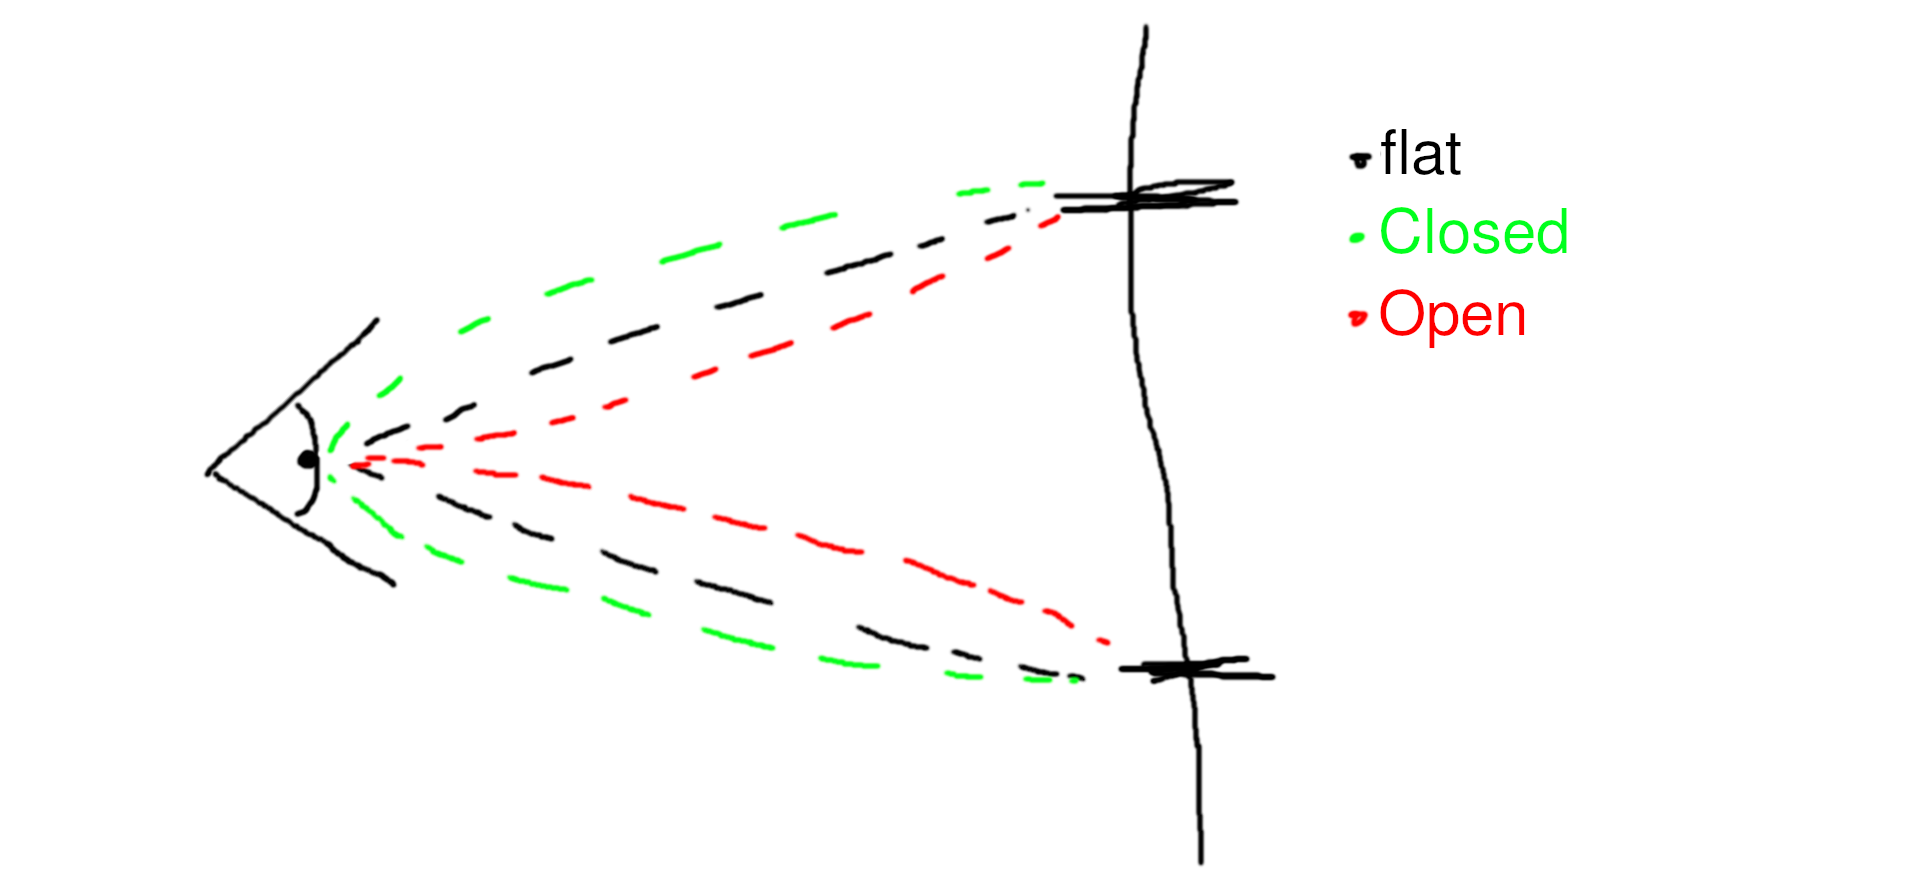
\includegraphics[scale=.5]{Universes.png}
\end{figure}
So if we know the spatial size of some feature on the last scattering surface you could use this relation to measure the curvature of the universe. And we could infer the spatial curvature from the location of the first peak in the power spectrum. So far we ignored the gravitational potential so let's now see what changes when we re-include $\Psi$:
We see from the equation (\ref{oscillations}) that it shifts the zero point of the oscillations by looking at the equilibrium point ($\ddot{\Theta} = \dot{\Theta} = 0 \implies \Theta_0^{eq} = - \frac{1}{3c_s^2}\Psi = -(1+R)\Psi$), i.e it enhances the odd over the even peaks:
\begin{figure}[h]
  \centering
  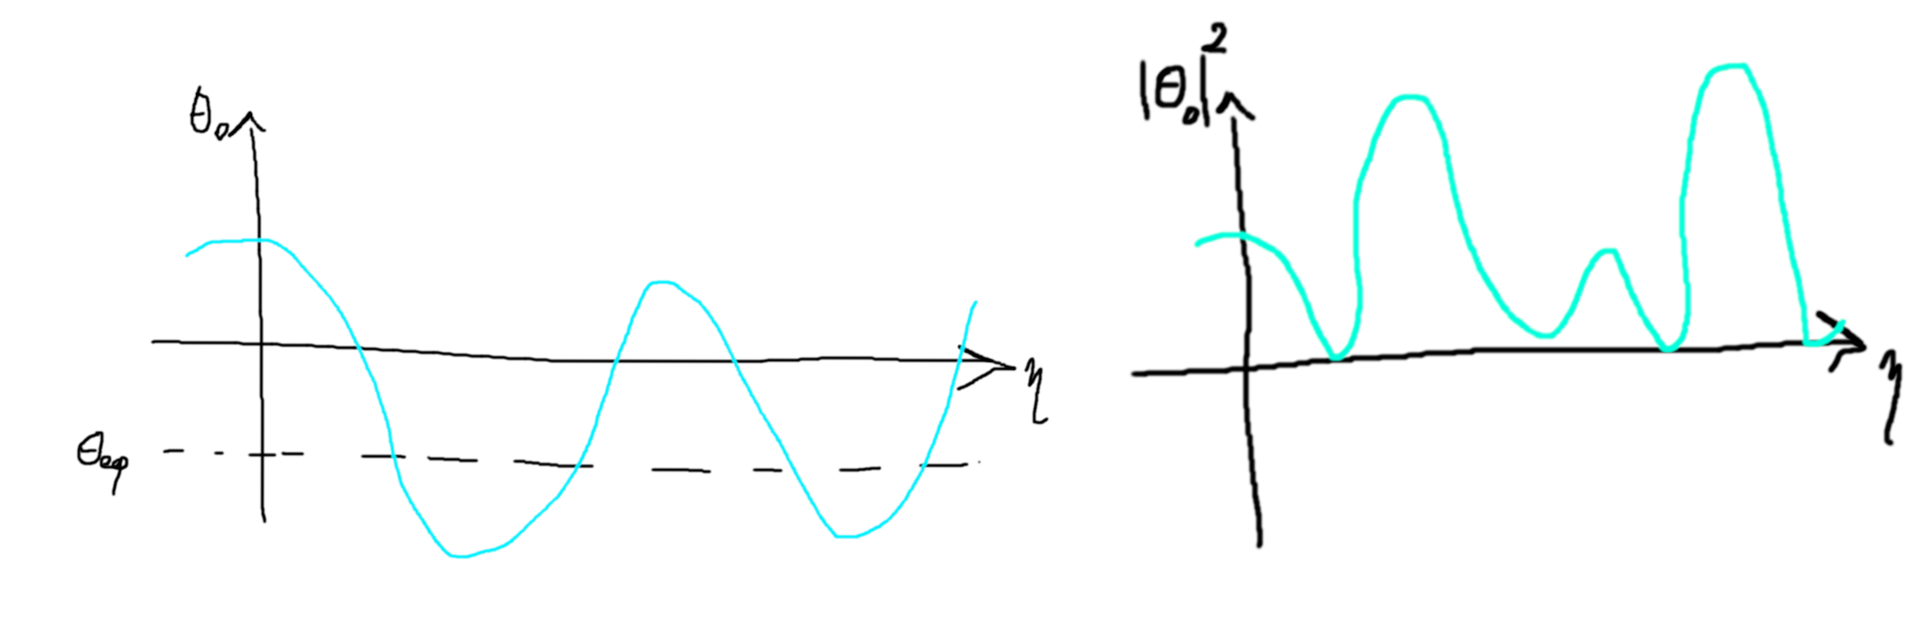
\includegraphics[scale=.5]{gravpot.png}
\end{figure}
We also see that the effect is stronger when the speed of sound is smaller, i.e when we have a high baryon fraction.So this is an effect that we can use to measure baryons in the universe! So for instance we can infer the amount of baryons from the height difference of the second to the first peak.
\\\\
The next interesting effect has to do with the decay of gravitational potentials which can give rise to a strong driving force, to see that look at the following analogy where the photon-baryon fluid is modeled by balls in a harmonic potential connected by a spring:
\begin{figure}[h]
  \centering
  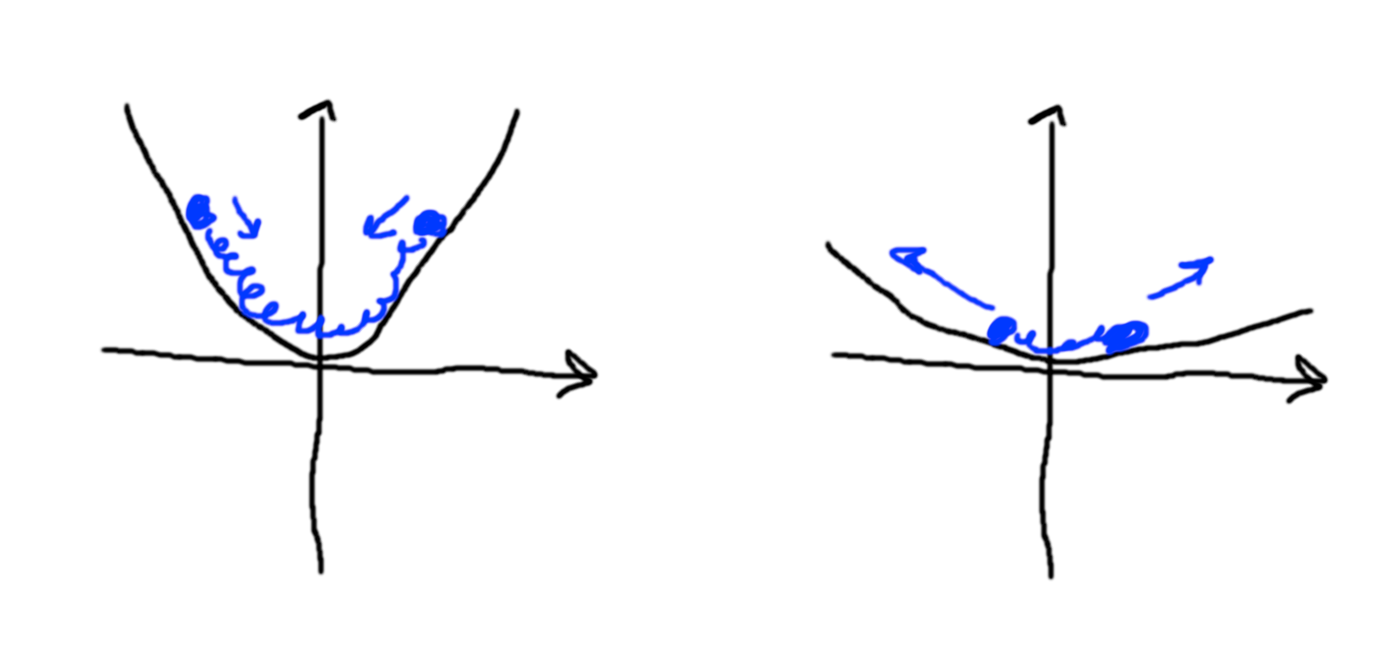
\includegraphics[scale=.5]{decaying.png}
\end{figure}\\
If in the compression phase the potential was stronger than in the subsequent decompression it's clear that on the way back the balls will overshoot and thereby cause oscillations of larger amplitudes. This happens for modes which enter the horizon during radiation domination, when the gravitational potentials decay inside the horizon.\\
If there's more dark matter then radiation domination stopped earlier $\implies$ less driving force $\implies$ lower peaks. I.e we can measure the amount of dark matter in the universe! To disentangle this from the previous ones we need to measure at least 3 peaks.\\\\

Now let's discuss diffusion damping: It turns out that the diffusion of photons just before decoupling leads to a surpression of the form 
\begin{equation}
  exp\left\{-\frac{l^2}{l_D^2}\right\}
\end{equation}
for small angle anisotropies where $l_D$ is related to the diffusion length, i.e damping of high peaks in CMB power spectrum. Now because this effect is related to the diffusion lenght which is related to the number of baryons, this effect can be used to independently measure the number of baryons in the universe! (consistency check)\\\\

Let's now say something about the ISW contributions, as they involve derivatives of the gravitational potentials, the contributions will come from regions in ($k,\eta$) space where metric fluctuations will vary in time. There are 2 such regions: 
\begin{itemize}
  \item Shortly after decoupling, on sub-soundhorizon scales (Early ISW effect) $\rightarrow$ increase first peak
  \item During $\Lambda$ domination (cosmological constant) (Late ISW effect) $\rightarrow$ increase lowest multipoles
\end{itemize}
So more dark matter $\implies$ less radiation left after decoupling $\rightarrow$ metric fluctuations decay less $\implies$ EISW contributes less $\implies$ lower first peak. So we can again measure the amount of dark matter with this.\\\\
Now let's discuss Reionization:\\
Reionization leads to re-scattering of photons at small redshift which tends to smooth out anisotropies ($z\approx 10$). It does so except on the largest scales $\implies$ decrease of $C_l$ for $l\geq 40$.
\section{Polarization}
So far we've only talked about temperature anisotropies which have to do with the energy carried by light but light also has polarization. Say we have a "cold" and a "hot" light source there will be a net polarization:
\begin{figure}[h]
  \centering
  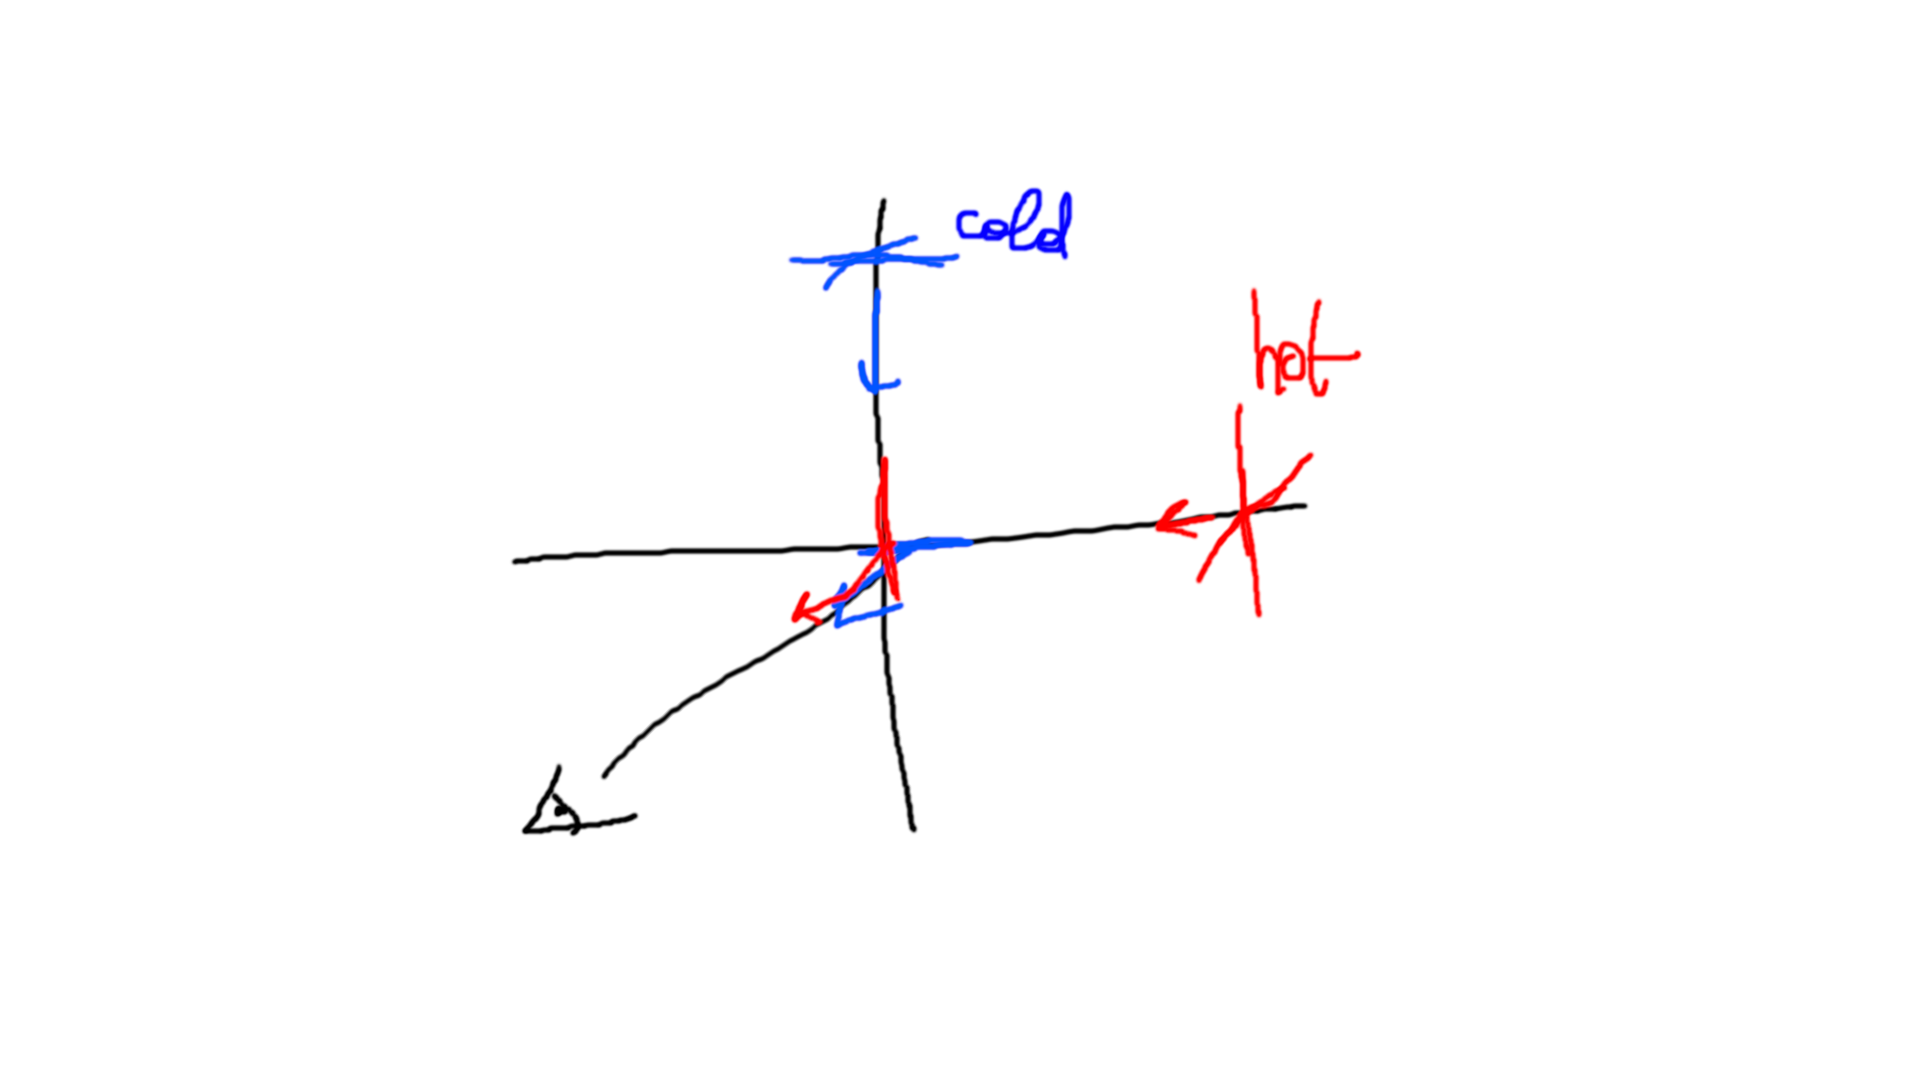
\includegraphics[scale=0.7]{polarization.png}
\end{figure}
So we see that polarization is due to Thomson scattering in the presence of a quadrupole.
Polarization can be represented by sticks of different size and orientation in different points of a map of the sky, those are related to the size and orientation of the quadrupole at each point on the last scattering surface.\\
These polarization modes can be decomposed in E\&B modes (As seen in electromagnetism), importantly scalar perturbations only produce E modes, whereas tensor perturbations produce both. So instead of just the temperature power spectrum $C_l^{TT}$ which we discussed so far, there's also a power spectrum of the E mode polarization $C_l^{EE}$, a cross correlation $C_l^{TE}$ and a pure $C_l^{BB}$ mode which hasn't been measured jet. As polarization is only produced by scattering there are 2 relevant periods:
\begin{itemize}
  \item recombination which affects small scales (in fact diffusion scale peaks at $l\approx 1000$) (at $\sim 10^{-6} K$ (which is a factor of 10 less than the temperature perturbations))
  \item reionization which affects large scales (at $\sim 10^{-7} K$)
\end{itemize}
Because of this last item, by measuring polarization on those large scales one can infer information about reionization. In particular one can use this to measure the optical depth to recombination $\tau_{reio}$.
What about Tensor modes? (primordial gravitational waves) On the one hand they would contribute to the temperature cpower spectrum $C_l^{TT}$ for $l\leq 100$ as gravitational waves decay quickly inside the hubble radius, so cosmic variance will be relatively important which prevents studying them in detail. Second tensor effect is on $C_l^{BB}$ which remains a big challenge!
\section{Cosmological parameters}
$\Lambda$CDM has a number of free parameters:
\begin{itemize}
  \item curvature density $\Omega_k \equiv 1 - \Omega_m - \Omega_\Lambda$
  \item baryon density $\Omega_b h^2$
  \item matter density $\Omega_m h^2$
  \item Cosmological constant energy density $\Omega_\Lambda$
  \item normalization $C_10$
  \item primordial tilt/slope n
  \item optical depth to recombination
  \item tensor modes $r\equiv \frac{C_2^T}{C_2^S}$ ("tensor-to-scalar ratio")
\end{itemize}
The tilt/slope is now: $n<1$ with high significance (i.e not scale-invariant). Often in cosmology the parameters are degenerate (we can't really measure a single parameter) e.g the tilt is degenerate with depth to recombination so it's important to break this degeneracy. One way of breaking it is by using polarization data.\footnote{The source code for this document can be found \href{https://github.com/arthuradriaens-code/Early-Universe-Cosmology/tree/main/CMB}{here}}
\end{document}
